\begin{solution}

\begin{enumerate}
\item {[7 points]} The code used to produce the results shown in this part and part~(b) is below.

\lstinputlisting{HW9ab.m}

Two acceptable styles of the desired plots are shown below. We also include $N=4$ for the sake of comparison.

\begin{center}
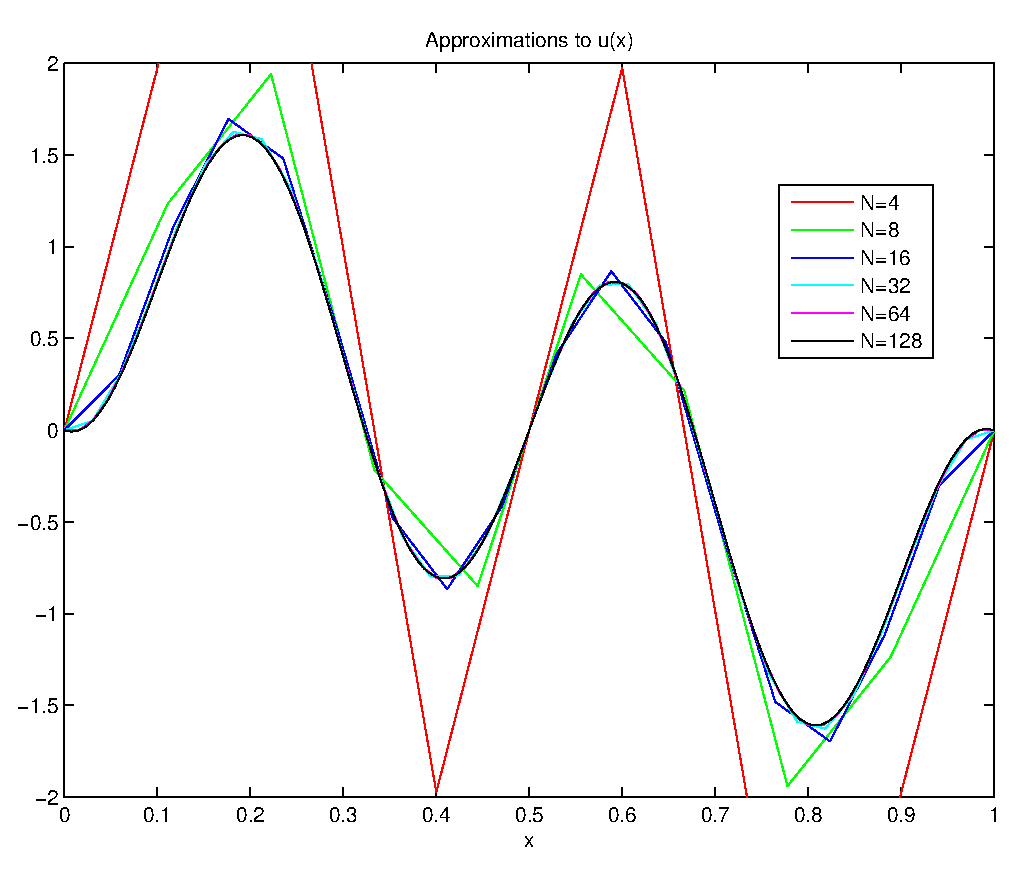
\includegraphics[scale=0.7]{together_a}
\end{center}

\begin{center}
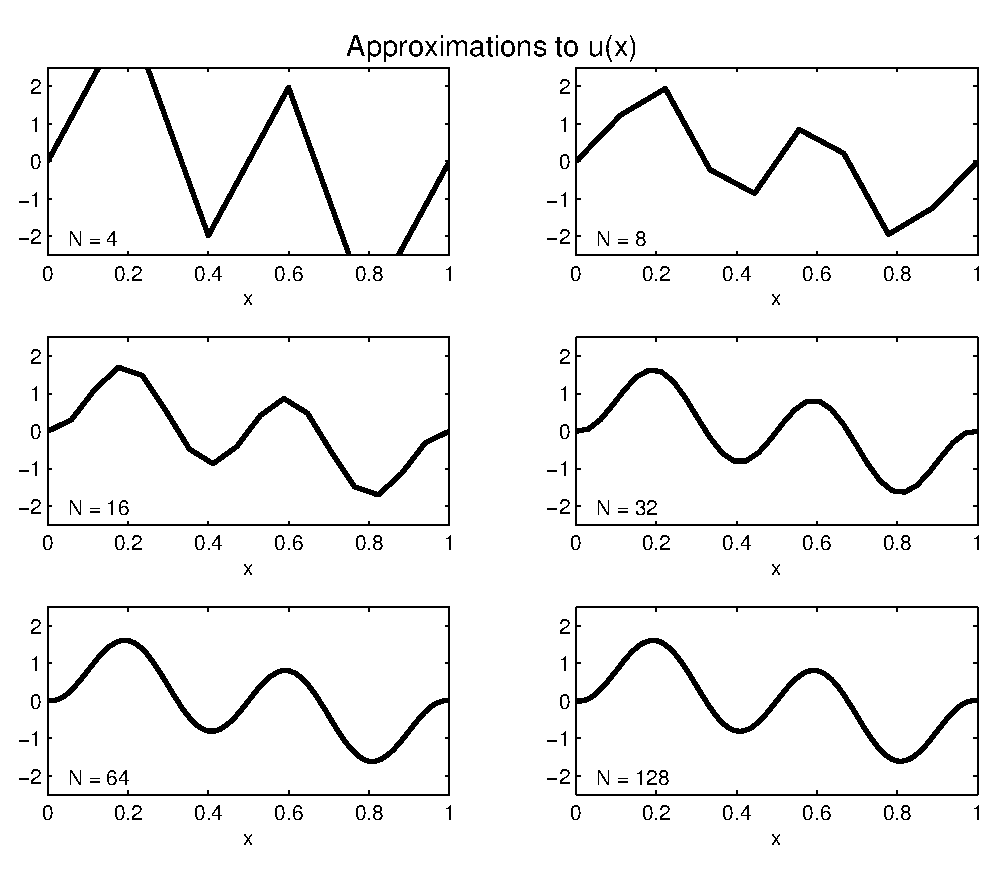
\includegraphics[scale=0.7]{separate_a}
\end{center}

\item {[5 points]} The desired plot is shown below.

\begin{center}
\includegraphics[scale=0.5]{error_b}
\end{center}

On the above plot, we include a line showing the rate of convergence
if the error was reduced exactly like $h^2$.  We see that the rates
(that is, the slope of the true error curve (solid) and this $h^2$
curve (dashed)) are quite close.  The follows from the fact that, for small enough $h$,
our approximation to the second derivative makes an error which is very nearly proportional to $h^2$.
\\
\item {[7 points]} 
Suppose we have $u(0) = \alpha$ and $u(1) = \beta$. The approximation to the second derivative 
\[
u''(x_j)\approx{u(x_{j-1})-2u(x_j)+u(x_{j+1})\over h^2},
\]
for $j=1,\ldots,N$, yields
\[ {1\over h^2} \left[\begin{array}{rrrrrrr}
              1 & -2 & 1 \\[0.25em]
               & 1 & -2 & 1 \\
                & &  1  & -2 & 1 \\
                & & & \ddots & \ddots & \ddots \\[0.25em]
                 && & & 1 & -2 & 1
               \end{array}\right]
          \left[\begin{array}{c} u(x_0) \\[0.25em] u(x_1) \\[0.25em] u(x_2) \\[0.25em] \vdots \\[0.25em] u(x_{N-1}) \\[0.25em] u(x_N) \\[0.25em] u(x_{N+1}) \end{array}\right]
 \approx   \left[\begin{array}{c} f(x_1) \\[0.25em] f(x_2) \\[0.25em] \vdots \\[0.25em] f(x_{N-1}) \\[0.25em] f(x_N) \end{array}\right].\]
Now,
\begin{eqnarray*}
&&{1\over h^2} \left[\begin{array}{rrrrrrr}
              1 & -2 & 1 \\[0.25em]
               & 1 & -2 & 1 \\
                & &  1  & -2 & 1 \\
                & & & \ddots & \ddots & \ddots \\[0.25em]
                 && & & 1 & -2 & 1
               \end{array}\right]
          \left[\begin{array}{c} u(x_0) \\[0.25em] u(x_1) \\[0.25em] u(x_2) \\[0.25em] \vdots \\[0.25em] u(x_{N-1}) \\[0.25em] u(x_N) \\[0.25em] u(x_{N+1}) \end{array}\right]
\\
&=&{1\over h^2} \left[\begin{array}{rrrrrrr}
              1 & -2 & 1 \\[0.25em]
               & 1 & -2 & 1 \\
                & &  1  & -2 & 1 \\
                & & & \ddots & \ddots & \ddots \\[0.25em]
                 && & & 1 & -2 & 1
               \end{array}\right]
         \left(\left[\begin{array}{c} 0 \\[0.25em] u(x_1) \\[0.25em] u(x_2) \\[0.25em] \vdots \\[0.25em] u(x_{N-1}) \\[0.25em] u(x_N) \\[0.25em] 0 \end{array}\right]
+
\left[\begin{array}{c} u(0) \\[0.25em] 0 \\[0.25em] 0 \\[0.25em] \vdots \\[0.25em] 0 \\[0.25em] 0 \\[0.25em] u(1) \end{array}\right]\right)
\\
&=&{1\over h^2} \left[\begin{array}{rrrrrrr}
              1 & -2 & 1 \\[0.25em]
               & 1 & -2 & 1 \\
                & &  1  & -2 & 1 \\
                & & & \ddots & \ddots & \ddots \\[0.25em]
                 && & & 1 & -2 & 1
               \end{array}\right]
         \left(\left[\begin{array}{c} 0 \\[0.25em] u(x_1) \\[0.25em] u(x_2) \\[0.25em] \vdots \\[0.25em] u(x_{N-1}) \\[0.25em] u(x_N) \\[0.25em] 0 \end{array}\right]
+
\left[\begin{array}{c} \alpha \\[0.25em] 0 \\[0.25em] 0 \\[0.25em] \vdots \\[0.25em] 0 \\[0.25em] 0 \\[0.25em] \beta \end{array}\right]\right)
\\
&=&{1\over h^2} \left[\begin{array}{rrrrrrr}
              1 & -2 & 1 \\[0.25em]
               & 1 & -2 & 1 \\
                & &  1  & -2 & 1 \\
                & & & \ddots & \ddots & \ddots \\[0.25em]
                 && & & 1 & -2 & 1
               \end{array}\right]
         \left[\begin{array}{c} 0 \\[0.25em] u(x_1) \\[0.25em] u(x_2) \\[0.25em] \vdots \\[0.25em] u(x_{N-1}) \\[0.25em] u(x_N) \\[0.25em] 0 \end{array}\right]
+
{1\over h^2} \left[\begin{array}{rrrrrrr}
              1 & -2 & 1 \\[0.25em]
               & 1 & -2 & 1 \\
                & &  1  & -2 & 1 \\
                & & & \ddots & \ddots & \ddots \\[0.25em]
                 && & & 1 & -2 & 1
               \end{array}\right]
\left[\begin{array}{c} \alpha \\[0.25em] 0 \\[0.25em] 0 \\[0.25em] \vdots \\[0.25em] 0 \\[0.25em] 0 \\[0.25em] \beta \end{array}\right]
\\
&=&{1\over h^2} \left[\begin{array}{rrrrr}
              -2 & 1 \\[0.25em]
               1 & -2 & 1 \\
                 &  1  & -2 & \ddots \\
                 & & \ddots & \ddots & 1 \\[0.25em]
                 & & & 1 & -2 
               \end{array}\right]
         \left[\begin{array}{c} u(x_1) \\[0.25em] u(x_2) \\[0.25em] \vdots \\[0.25em] u(x_{N-1}) \\[0.25em] u(x_N) \end{array}\right]
+
\left[\begin{array}{c} \alpha/h^2 \\[0.25em] 0 \\[0.25em] \vdots \\[0.25em] 0 \\[0.25em] \beta/h^2 \end{array}\right]
\end{eqnarray*}
and so
\[ {1\over h^2} \left[\begin{array}{rrrrr}
              -2 & 1 \\[0.25em]
               1 & -2 & 1 \\
                 &  1  & -2 & \ddots \\
                 & & \ddots & \ddots & 1 \\[0.25em]
                 & & & 1 & -2 
               \end{array}\right]
         \left[\begin{array}{c} u(x_1) \\[0.25em] u(x_2) \\[0.25em] \vdots \\[0.25em] u(x_{N-1}) \\[0.25em] u(x_N) \end{array}\right]
 \approx   \left[\begin{array}{c} f(x_1) \\[0.25em] f(x_2) \\[0.25em] \vdots \\[0.25em] f(x_{N-1}) \\[0.25em] f(x_N) \end{array}\right]-\left[\begin{array}{c} \alpha/h^2 \\[0.25em] 0 \\[0.25em] \vdots \\[0.25em] 0 \\[0.25em] \beta/h^2 \end{array}\right].\]

Hence, we can approximate the differential equation
\[ u''(x) = f(x), \quad 0<x<1,\]
with inhomogeneous Dirichlet boundary conditions
      \[ u(0)=1,\quad  u(1)=2\]
by the matrix equation
\[ {1\over h^2} \left[\begin{array}{rrrrr}
              -2 & 1 \\[0.25em]
               1 & -2 & 1 \\
                 &  1  & -2 & \ddots \\
                 & & \ddots & \ddots & 1 \\[0.25em]
                 & & & 1 & -2 
               \end{array}\right]
          \left[\begin{array}{c} u_1 \\[0.25em] u_2 \\[0.25em] \vdots \\[0.25em] u_{N-1} \\[0.25em] u_N \end{array}\right]
 =   \left[\begin{array}{c} f(x_1)-1/h^2 \\[0.25em] f(x_2) \\[0.25em] \vdots \\[0.25em] f(x_{N-1}) \\[0.25em] f(x_N)-2/h^2 \end{array}\right],\]
where $u_j \approx u(x_j)$.  (Entries of the matrix that are not specified are zero.)
\\
\item {[6 points]} The code below produces two acceptable styles of the requested plots, plus a few extra.

\lstinputlisting{HW9d.m}

Two acceptable styles of the  requested plots, plus a few extra, are below.

\begin{center}
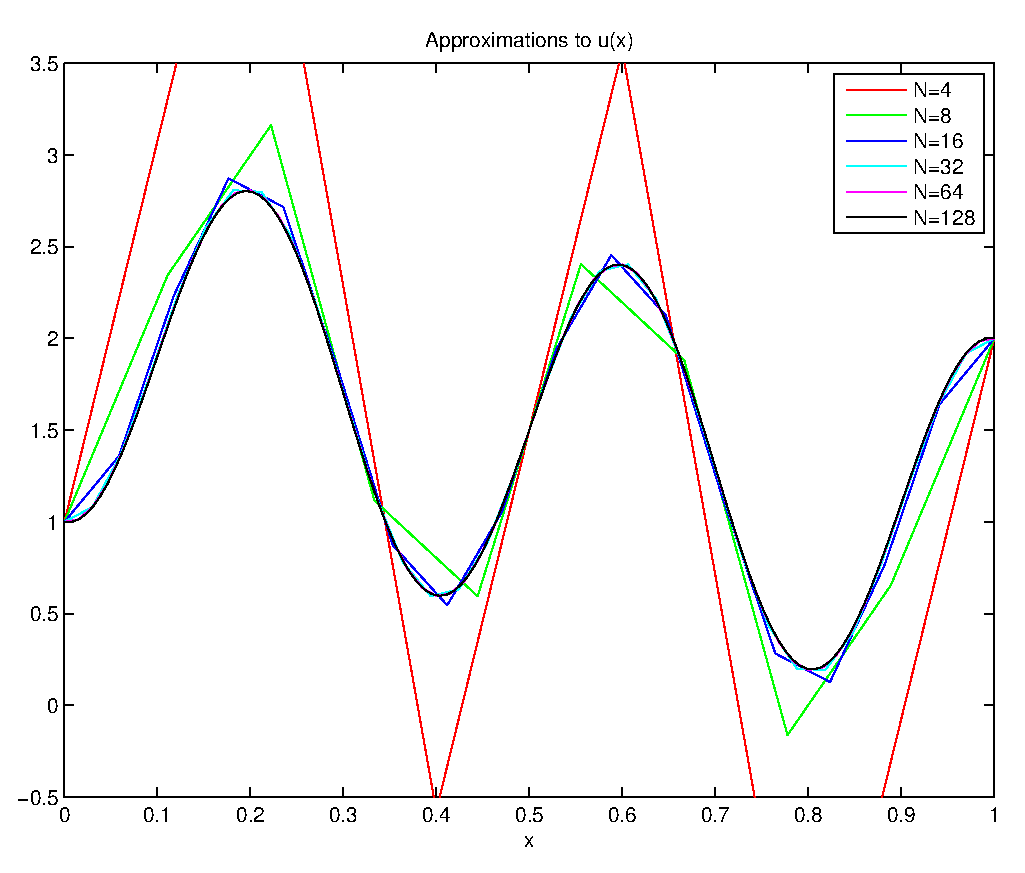
\includegraphics[scale=0.7]{together_d}
\end{center}

\begin{center}
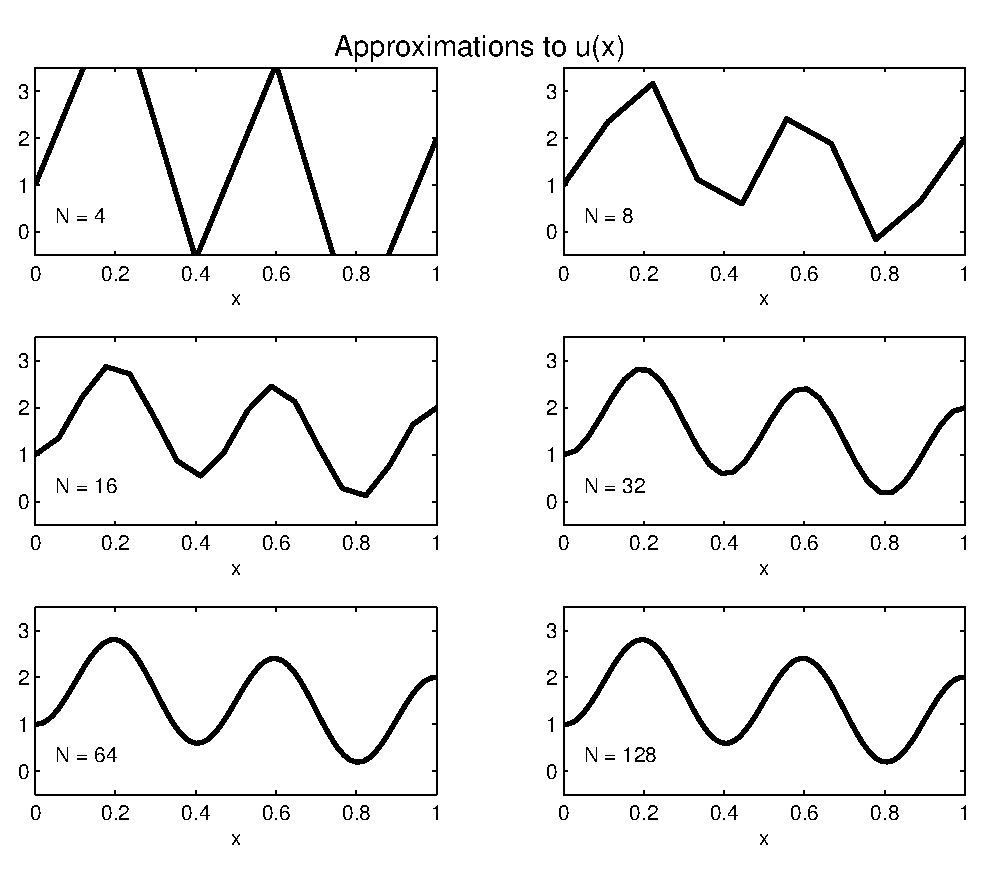
\includegraphics[scale=0.7]{separate_d}
\end{center}

\end{enumerate}
\end{solution}
